% 来源：OEBPS/Text/Section0001_split_006.xhtml#sigil_toc_id_45

\BookChapter{32}
\section[第32章\q 卡尔·伊坎：宇宙主宰]{第32章\\ 卡尔·伊坎：宇宙主宰}

\begin{figure}[htbp]
\centering
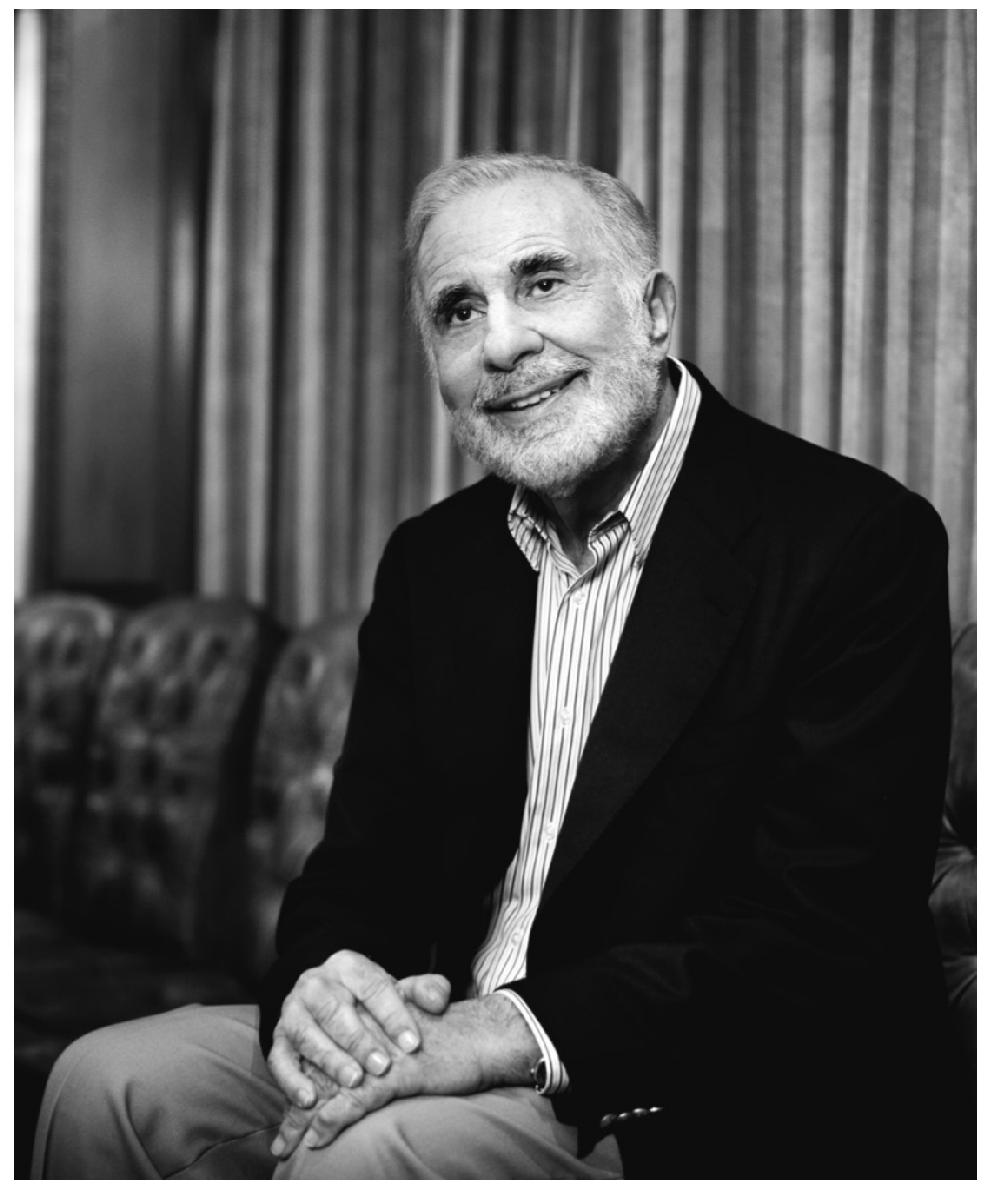
\includegraphics[width=0.43\linewidth,keepaspectratio]{image/卡尔·伊坎肖像.jpg}
\caption*{卡尔·伊坎}
\end{figure}

华尔街上最让人害怕的人

问：什么时候发一条微博能价值170亿美元？

答：卡尔·伊坎发微博说，苹果公司的股票被低估了，他宣布自己正在买入苹果股票。

2013年夏，卡尔·伊坎发了这条微博，之后不到一个小时，苹果股价跃升0.19\%。股票市场明白这条微博背后的意思：什么时候这个身家百亿的投资家对一家公司的股票有兴趣，那时就是你买入的好时机。4个月后，《时代》杂志把卡尔·伊坎作为封面人物，标题是《宇宙主宰》。这名号封得有些大了。文章里面说他是“美国最重量级的投资人”。这话说得对。在过去40年里，卡尔·伊坎的公司赚的钱要比另一位投资大师沃伦·巴菲特的公司高出50\%。《吉普林》个人理财杂志上有篇文章分析道，尽管大多数人都认为巴菲特的长期投资业绩是最好的，但是如果你在1968年投资卡尔·伊坎控股的公司，到2013年，你持有45年得到的复利年化收益率为31\%，而沃伦·巴菲特控股的公司伯克希尔–哈撒韦公司的同期年化收益率“只有”20\%。

卡尔·伊坎高超的投资和经营技巧让他成为世界上最富有的人之一，根据最新一期《福布斯》400富豪排行榜，他排名第27，个人财富净值超过230亿美元，他给伊坎公司的股东的钱更多。伊坎公司在纳斯达克上市，股票代码是IEP，是一家多元化的控股公司。持有伊坎公司的股票，就能跟着卡尔·伊坎这位投资大师赚大钱，或者去买卡尔·伊坎盯上的要收购公司的股票，它们往往后来会大涨，也能让你赚到很多钱。卡尔·伊坎投资成功的秘诀是什么？即使是他的批评者也会告诉你，卡尔·伊坎不仅是寻找机会，他还制造机会。

但是大多数投资外行仍旧把他看作华尔街上的秃鹫，一个残酷无情的资本家，袭击并购上市公司，大肆掠夺，肥了自己的腰包。你在谷歌上搜索“公司袭击者”，卡尔·伊坎的名字便会自动出现在搜索框里。

但是，卡尔·伊坎是在挑战传统的腐朽观念。卡尔·伊坎把自己看作一个“股东维权者”，这是什么意思？“我们购买股票，进入上市公司，告诉管理者真相：你们并没有创造出股东应得的价值。”他告诉我。他说，他痴迷的事情是让上市公司停止虐待股票，为此要改善公司管理，加强公司问责，这样做能让美国公司更加强大，从而让美国经济更加强大。

《纽约时报》这样描述他：“威逼公司董事会做决策，积累控制公司的实力，大力推动公司进行改革，这让卡尔·伊坎建立了数十亿美元的财富，但在上市公司高管中激起了一片恐惧，同时在这个过程中，此举在追随他的众多投资者中也激起了一片崇拜。”

卡尔·伊坎大量买进投资过多或者业绩低于预期水平的上市公司股票，然后提醒公司董事会和高管注意，现在该加快前进速度好好表现了，否则他们就要面对争夺董事会控制权的战争。

他把自己看作一个斗士，那些高管运用上市公司的宝贵资源，肥了自己的腰包，而让股东们为此付出代价，他就是要跟这些吃里爬外的高管斗。“托尼，那些股东根本不知道他们吃了这些高管的大亏。”卡尔·伊坎对我说，再加上一般投资者根本不知道，在董事会关上门的背后，那些高管滥用股东赋予的权力，做出的决策是损害股东利益的。但是，有一部分原因是股东并不认为他们有能力改变现状，因为他们并不像企业所有人一样思考。可是卡尔·伊坎知道杠杆的巨大力量，而且他并不害怕使用杠杆。

有些上市公司董事会采取的行动会惹怒卡尔·伊坎，其中的一个例子是他猛烈地批评可口可乐公司。这是因为可口可乐公司决定，折价发行价值240亿美元的新股，但这样会稀释公司的股票价值。为什么要这样做？为了筹集巨资对公司高管进行股权激励，这将会削弱普通投资者的退休金投资收益，其中包括教师和消防员，因为很多人都在退休金投资组合里持有可口可乐公司的股票。

卡尔·伊坎在《巴伦周刊》上写了一篇评论文章，猛烈抨击可口可乐公司这项股票发行计划，而且批评沃伦·巴菲特没有投票反对公司这个举动，因为巴菲特控股的伯克希尔–哈撒韦公司是可口可乐公司的最大股东，巴菲特也是可口可乐公司董事会成员。“太多董事会成员都把董事会当作大学生联谊会或者俱乐部了，在那里你一定不要批评别人。”卡尔·伊坎写道，“正是这种不得罪人的态度助长了管理层的平庸。”

巴菲特回应道，他放弃了投票，但他是反对这个计划的，他已经平静地跟管理层谈过了，付给管理层的股权激励过高，应该降低，但是巴菲特在这个问题上不想和可口可乐公司“开战”。

相反，卡尔·伊坎随时准备开战，他已经多次在战壕里和很多公司开战了。这些公司的范围很广，包括美国钢铁公司、高乐士、亿贝、戴尔、雅虎。但是这一次不同，不是卡尔·伊坎，而是一个年轻的基金经理，名字叫戴维·温特斯，他正在买入股票，然后众人开始控告可口可乐公司管理层。由于看不惯付给首席执行官的薪酬过高的现象，新一代“维权投资者”接过了卡尔·伊坎的枪，要把他几十年前发起的战斗继续打下去。

自然而然地，卡尔·伊坎也惹怒了一大帮企业大佬，他的这些敌人在媒体上有很大的影响力。所以，你经常可以听到媒体对卡尔·伊坎的批评，说他干这事只是为了钱，或者说他“先建仓后推高股价再压低股价出货”，以牺牲公司的长远目标来换取短期的盈利，但是卡尔·伊坎指出，这种说法简直荒谬可笑，因为他经常持有股票很长时间，比大家认为的要长得多，有的时候持有时间长达10年、15年，甚至30年。他获得一家上市公司的控制权之后，这家公司的市场价值会持续上涨好多年，甚至在他抛掉股票离场之后依然如此。这种说法得到了研究证实，哈佛商学院的教授卢西恩·拜伯切克做了一项调查研究，分析了2000个股东的维权行动，时间从1994年到2007年共14年，分析得出的研究结论是：“股东维权者介入之后，公司经营业绩得到改善。”这项研究还发现，股东维权不但没有破坏性的长期效应，相反，5年后这些公司的经营业绩出色。

卡尔·伊坎并不是对每个上市公司的首席执行官都进行攻击，他承认确实有一些非常杰出的公司管理团队，这些公司高管最大限度地利用公司资源，让公司的经营更有活力。但是他始终在寻找一些方法，让管理层对股东更加负责，即使是最流行而且管理很好的公司管理层。

比如卡尔·伊坎发那条关于苹果公司的微博，他告诉我，他并不是想要推高股价，为了把自己手里的股票高价卖掉。（事实上，在我们对话的那一天，他又买进了很多苹果股票。）卡尔·伊坎并不想插手苹果公司的管理，他觉得公司的管理很稳固。卡尔·伊坎发这条微博，只是他搞的这场战役中的一场战斗而已，他的这场战役是向苹果公司施压，把1500亿美元的现金储备的全部分红还给股东。苹果公司最终在2014年4月扩大了原来的资本收益计划，规模超过1300亿美元，其中包括提高股票回购授权，从原来宣布的600亿美元提高到900亿美元。与此同时，苹果公司宣布提高季度分红，然后进行7股合成1股的股票反向拆分。现在，和他发出微博那天相比，苹果公司的股价上涨了50\%。

卡尔·伊坎本人也是一位首席执行官，持有伊坎公司这家上市公司88\%的股份。这家公司的股票市场表现简直好得惊人，即使是在过去所谓失落的十年，它也涨得很好。如果你在2000年1月1日买入伊坎公司的股票，那么到2014年7月31日，你能赚到1622\%的总收益率，相比之下，同期标准普尔500指数的收益率只有73\%。

卡尔·伊坎并不是一生下来就过上这种生活的。他说，他是在纽约法洛克威“街头”长大的，他的妈妈是一名老师，他的爸爸原来在大学里学法律，后来成了一个不成功的歌剧演员，在当地的犹太教堂的唱诗班做领唱。卡尔·伊坎靠玩扑克牌赢钱支付自己读普林斯顿大学的学费和生活费，他读的专业是哲学。大学毕业后，他先到一家医疗学校干了很短一段时间，又到部队里干了一段时间（主要就是打牌），他逐渐意识到自己最大的才能是赚钱。每一副扑克牌都是一样的，但美国上市公司从来不是一样的。

写本书时，卡尔·伊坎78岁，他在考虑他要给后人留下什么样的遗产，他一直忙着写评论文章，也有选择性地接受一些采访，谈谈关于投资者和股东的维权。但是坦白地说，他大概烦透了别人误解他的话，断章取义地引用他说的话。这也正是为什么他一开始在不知道我是什么样的人，也不知道我真正的意图是什么时，他不许我们拍摄访谈过程，而且直接声明：“我只给你几分钟。”

让我感到长舒一口气的是，虽然刚开始气氛有点儿尴尬，但是过了一小段时间后，卡尔·伊坎就像做了热身运动一样开始活跃起来，我们一直聊了两个半小时，之后我和他在大堂里散步，他还把我引荐给他的妻子盖尔，她是位非同寻常的女士，他们已经结婚15年了。卡尔·伊坎本人实际上跟他的公众形象差别很大，他幽默风趣，又很好奇，甚至有点儿像个慈祥的老爷爷。朋友们都说他现在比以前温和多了。但是他说话还带着纽约皇后区的口音，而且他依然带有纽约街头跟人吵架的那种锋芒。卡尔·伊坎说，他可不是那种会放弃的家伙，特别是他发现有种东西值得去战斗时。

\begin{BookQuote}
\textbf{罗宾斯：}你出身于一个条件一般的家庭，在皇后区的一个贫困地区，你上的是公立学校。最开始，你有没有设立一个目标，要成为历史上最优秀的投资者？
\end{BookQuote}

\begin{BookQuote}
\textbf{卡尔·伊坎：}我是竞争欲望很强的人。很有激情或者说很痴迷，不管你怎么说。不管我干什么，我都要成为最好的那一个，这是我的天性。我申请读大学的时候，我的老师说：“你就别费事去申请那些重点名校了，它们根本不会要我们这些来自贫困地区的孩子。”我仍然坚持参加了大学入学考试。结果多所重点名校都录取我了。我从中选择了普林斯顿大学。本来我父亲答应了，如果我考上名牌大学，所有的费用都由他来付。后来他却说话不算数了，只帮我付了学费，你相信吗？那个时候一年只要750美元。我说：“你这个父亲说话不算数，不给我生活费，我睡哪儿，我吃什么？”我的父亲说：“你这么聪明，你会想到办法的。”
\end{BookQuote}

\begin{BookQuote}
\textbf{罗宾斯：}那你是怎么解决的？
\end{BookQuote}

\begin{BookQuote}
\textbf{卡尔·伊坎：}打工呗。我在新泽西洛克威的一家俱乐部里找到一份工作——当个沙滩男孩。我是个很棒的沙滩男孩。沙滩上那个更衣室的老板经常招呼我：“嘿，小伙子，快过来跟我们打扑克牌吧，我要把你这个星期挣的小费都赢光。”一开始我根本不知道怎么玩扑克牌，他们把我的钱赢了个干干净净。我这个人从来不服输，我一个名校大学生难道还玩不过你们！于是我借了三本讲玩扑克牌技巧的书，花了两个星期仔细阅读，从此我的牌技比他们都要高上10倍，我当然经常赢了。当时我觉得那真是个大游戏，赌注很大。每年夏天我都能赢差不多2000美元，你要知道，那可是在20世纪50年代，那时候的2000美元抵得上现在的5万美元。
\end{BookQuote}

\begin{BookQuote}
\textbf{罗宾斯：}那你在商业投资上是怎么起步的？
\end{BookQuote}

\begin{BookQuote}
\textbf{卡尔·伊坎：}大学毕业后，我去参军，在部队里我继续玩扑克牌赌钱。等我离开部队的时候，攒了2万美元。我开始在华尔街做投资，那是1961年。当时我的生活过得很好了，还找了一个很漂亮的模特做女朋友，我买了一辆白色的敞篷银河跑车。结果1962年股市崩盘了，我的所有东西都亏掉了。我不知道是哪个先跑的，可能是我的女朋友，也可能是我的跑车！
\end{BookQuote}

\begin{BookQuote}
\textbf{罗宾斯：}我看过关于你的报道，说你后来重新回到了投资市场，卖期权，然后又开始做套利交易。
\end{BookQuote}

\begin{BookQuote}
\textbf{卡尔·伊坎：}我借钱去纽约股票交易所买了个席位，我是艺高人胆大的家伙。我的经验教会了我，在股市上做短线交易很危险，不如发挥我的数学能力，在某方面成为专家，这肯定要好得多。我做套利交易，银行愿意贷给我90\%的资金，因为那个时候我做的是根本没有风险的套利交易，如果做得好的话，我基本上不可能亏钱。从这以后我就开始赚大钱了，一年能赚150万\textasciitilde{}200万美元。
\end{BookQuote}

\begin{BookQuote}
\textbf{罗宾斯：}我很想请教你一下风险—收益不对称。当时你开始收购股票价格被低估的公司的控制权时，你是不是也在寻找风险—收益不对称的机会？
\end{BookQuote}

\begin{BookQuote}
\textbf{卡尔·伊坎：}我开始仔细研究这些公司，认认真真地分析。我告诉你，这有点儿像是套利交易，但是没有人喜欢做这种事。你要是收购了一家公司，你真正买到手的是公司的资产，所以你要好好看看这些公司的资产，认真问问自己：“它们本来应该做得不错，为什么它们做不到？”整体来看，有90\%的可能性，问题出在管理上。所以我们会去寻找那些经营管理做得不好的公司，我有足够多的资金，我能够大量买入这家公司的股票，然后警告这家公司的董事会：“你要是不改变的话，我就收购你们公司，拿走控制权，除非董事会做到我说的一二三条。”大多数时候这家公司的董事会会说“好的”，但是有的时候，公司管理层会跟我斗，可能还会斗到法庭上。很少有人有我这么大的韧性，也很少有人像我这样愿意拿大钱去冒险。你看看这个局面。可能你会觉得我拿了很多钱在冒险，但是其实我根本没有。
\end{BookQuote}

\begin{BookQuote}
\textbf{罗宾斯：}但是你并不觉得这是冒险，因为你知道公司资产的真实价值。
\end{BookQuote}

\begin{BookQuote}
\textbf{卡尔·伊坎：}你在到处寻找风险—收益比，对不对？每一件事既有风险又有收益，但你必须要明白风险是什么，也要明白收益是什么。很多人看到的风险要比我多得多。但是数字不会撒谎，他们就是没有算明白。
\end{BookQuote}

\begin{BookQuote}
\textbf{罗宾斯：}为什么他们算不明白？
\end{BookQuote}

\begin{BookQuote}
\textbf{卡尔·伊坎：}因为有太多变量，太多分析，可能会动摇你的看法。
\end{BookQuote}

\begin{BookQuote}
\textbf{罗宾斯：}现在这些日子，那些上市公司的高管严防恶意收购，你要击败他们比以前更难。
\end{BookQuote}

\begin{BookQuote}
\textbf{卡尔·伊坎：}其实并非如此。现在美国这套体制是有缺陷的，你没办法把那些业绩平庸的经理人赶走。举个例子，我继承了一个很好的酒庄，在一块美丽的地方，有一片美丽的葡萄园。过了半年，我想卖掉它，因为这个酒庄不赚钱。但是我碰到了问题，管理这个酒庄的那个家伙从不来葡萄园上班。他整天到处打高尔夫球，可是他又不愿意放弃这份管理酒庄的工作，因为这会减少他一大笔收入。他不想让任何人进来看这个酒庄，因为他不想看到酒庄被卖掉。你也许会对我说：“你怎么回事啊，你傻了？把警察叫来，让他离开！”但是，要是上市公司就麻烦大了：不经过一场非常艰苦的斗争，你不可能做到让管理层走人。
\end{BookQuote}

\begin{BookQuote}
\textbf{罗宾斯：}法律法规有太多障碍，让你很难在自己控制的公司把首席执行官踢走。
\end{BookQuote}

\begin{BookQuote}
\textbf{卡尔·伊坎：}麻烦就在这里。上市公司的股东想让管理层听到自己的意见，有非常大的困难，但是我们伊坎公司会去斗争，也经常获胜。一旦掌握了上市公司的控制权，有的时候我们发现，其实管理层也不是那么糟糕。但是关键在于上市公司的治理方式，对于这个国家来说实在是太糟糕了。美国有很多法律法规，让你无法成为一个积极维权的股东。你要获得上市公司的控制权有很多障碍，但是一旦我们拿到控制权，所有股东的一般收益都会非常好，历史业绩记录也证明了这一点。除此之外，我们做的事，对美国经济也非常好，因为这让公司生产效率更高，而且这不仅仅是短期的效应。有的时候我们会一直持股不卖，持有股票长达15\textasciitilde{}20年。
\end{BookQuote}

\begin{BookQuote}
\textbf{罗宾斯：}你有什么解决方案？
\end{BookQuote}

\begin{BookQuote}
\textbf{卡尔·伊坎：}废除那些毒丸计划（公司高管发现有个股东买的股票太多了，怕他收购公司，他们就会折价发行很多股票，来稀释这个股东的股权比例），废除那些令人震惊的董事选举，让股东能够决定他们想让谁来管理公司。我们应该让这些公司高管真正对股东负责，进行真正的选举。即使是在政治上，尽管美国政治体系相当糟糕，但只要选民愿意，他们还是可以摆脱那些烂总统的。总统再烂，最多不过是在那一届干上四年，连选不上，就会下台走人。但是，在上市公司中，即使那个当首席执行官的家伙做的工作非常糟糕，你作为股东，要换掉这个烂首席执行官，也非常困难，比美国选民要换掉美国总统还难。这些首席执行官就像在大学里学生会的会长一样，他们并不是最聪明的家伙，但是他们是最会搞社交的，是最受大家喜欢的，所以他们才能一级一级地爬到最高的位置。
\end{BookQuote}

\begin{BookQuote}
\textbf{罗宾斯：}有的时候你并不需要发动一场代理权战争来改变公司的发展方向。例如，最近你买了很多网飞公司的股票，股权占比接近10\%，让你两年就赚了20亿美元。
\end{BookQuote}

\begin{BookQuote}
\textbf{卡尔·伊坎：}那都是我儿子布雷特和他的合伙人干的。我对高科技不太了解，但是，我儿子只用20分钟就给我讲明白了，为什么这是一笔好买卖。我只说了一句：“能买多少就买多少！”这其实并不是那种股东维权的投资。
\end{BookQuote}

\begin{BookQuote}
\textbf{罗宾斯：}你看到了什么东西？你儿子在那20分钟里展示给你的是什么东西，让你判定这只股票股价被过分低估了呢？
\end{BookQuote}

\begin{BookQuote}
\textbf{卡尔·伊坎：}很简单。大多数杰出的专家都很担忧那些错误的东西。就在那个时候，网飞公司每年能进账20亿美元的订阅费，但是这些收费并没有显示在公司的资产负债表上。因此所有这些专家都在问：“网飞公司怎么能搞到那么多钱去购买播放内容？”很简单，它有20亿美元的订阅费进来啊！一般来说，网飞公司的订阅用户都很忠诚，留下来继续订阅的时间比你想象的还要长！不管发生什么情况，要搞得如此巨大的现金流陷入危险的境地，都需要很长的时间，要比大多数人想象到的时间长得多。
\end{BookQuote}

\begin{BookQuote}
\textbf{罗宾斯：}但是你从来没有打算夺取网飞公司的控制权吗？
\end{BookQuote}

\begin{BookQuote}
\textbf{卡尔·伊坎：}网飞公司的高管认为，他们会有一场代理权大战，我肯定想要夺走公司的控制权。但是我说：“里德（网飞公司的联合创始人兼首席执行官），我不会跟你搞一场代理权大战。因为你有个举动刚刚在我这里得到了100分。”他听得一头雾水。我问他，你知不知道伊坎规则。他们说：“不知道，请问它是什么？”我说：“伊坎规则就是只要三个月不能赚到8个亿，我就会一拳打得他满嘴出血。”
\end{BookQuote}

\begin{BookQuote}
\textbf{罗宾斯：}（哈哈大笑）我看到，快到2013年年底的时候，你把一部分网飞公司的股票卖出变现了。
\end{BookQuote}

\begin{BookQuote}
\textbf{卡尔·伊坎：}股价涨到350美元的时候，我决定卖掉一部分股票，落袋为安，但是我并没有全部卖掉。
\end{BookQuote}

\begin{BookQuote}
\textbf{罗宾斯：}你觉得大家对你最大的误解是什么？
\end{BookQuote}

\begin{BookQuote}
\textbf{卡尔·伊坎：}我想，也许是大家不明白，也许是我自己不明白，我自己的动机到底是什么。也许这听起来很像陈词滥调，但是我确实在想，我的年龄到了70多岁，我很想做些事情，让我的国家更加强大。我希望留给后人的遗产是我改变了公司做生意的方式。这件事一直困扰着我，美国有这么多非常伟大的公司，却管理得那么糟糕，我想改变规则，让公司的首席执行官和董事会真正地对股东负责。
\end{BookQuote}

\begin{BookQuote}
\textbf{罗宾斯：}你和你妻子签订了给予誓言，要把大部分财产捐赠给慈善事业。除此之外，还有其他什么类型的慈善活动让你充满激情，非常投入？
\end{BookQuote}

\begin{BookQuote}
\textbf{卡尔·伊坎：}我给予了很多，但是我喜欢由自己来做。我刚刚捐赠了3000万美元给私立学校，因为在这些私立中小学校，校长和老师都很尽职尽责。一家私立学校，如果经营管理得好，会给我们的孩子更好的教育，它比公立学校强多了。美国是个伟大的国家，但很悲哀的是，我们经营管理公司的方式、我们管理教育体系的方式，在很大程度上是功能失调的。我希望能够运用我的财富，让我成为改变这种现状的一股力量。可悲哀的是，我们如果不这样做，这样一路发展下去，就会成为一个二流国家，甚至是三流、四流国家。
\end{BookQuote}

\subsection[投资要点]{投资要点\footnote{\label{fn:pdf-32-1}数据来源于彭博资讯，包括红利再投资。根据2014年7月31日收盘价计算。}}

卡尔·伊坎相信，对于主动型投资者来说，如果操作正确的话，再没有比今天更好的投资时机了。

这个看法主要基于以下因素：

\begin{itemize}
\item 利率水平低，这让并购成本降低，相应会提高并购投资收益率，让并购更有吸引力。
\item 现在有很多现金丰富，能从并购的协同效应中大大受益。
\item 很多机构投资者现在普遍意识到，现在很多上市公司高管能力平庸，董事会根本不关心股东，这种普遍现象必须处理，否则美国就无法终止高失业率，在世界市场上保持竞争力。
\end{itemize}

但是要让并购发生，需要一个股东维权者作为催化剂：

\begin{itemize}
\item 伊坎公司花了好多年建立并完善股东维权模式，我们相信，推动高增值型并购和合并事件就是需要的催化剂。
\item 可以推断，低利率水平将会大大增加伊坎公司控制的公司能力，运用我们的股东维权专长，做出公正的、善意的或者不是那么善意的并购。
\end{itemize}

\subsection[创造超一流业绩的可靠历史记录]{创造超一流业绩的可靠历史记录\footnote{\label{fn:pdf-32-2}收益计算按照2014年6月30日收盘价。}}

伊坎公司的股票从2000年1月1日以来累计涨幅为1622\%。

\begin{itemize}
\item 同期标准普尔500指数上涨73\%，道琼斯指数上涨104\%，罗素2000指数上涨168\%。
\end{itemize}

伊坎投资基金从2004年11月创立以来的业绩表现：

\begin{itemize}
\item 总收益率293\%，年化复合收益率15\%。
\item 年度业绩：2009年33.3\%，2010年15.2\%，2011年34.5\%，2012年20.23\%\footnote{\label{fn:pdf-32-3}收益计算假设伊坎公司持有的CVR能源股票整个期间都在投资基金里面。伊坎公司是在2012年5月获得CVR大多数股权。在CVR能源变成一个统一的实体之后剔除CVR能源的收益，投资基金的收益率约为6.6\%。}，2013年10.2\%，2014年年初至今30.8\%\footnote{\label{fn:pdf-32-4}截至2014年6月30日的前6个月。}。
\end{itemize}

\subsection{最近的财务数据}

2014年截至6月30日前6个月，归属于伊坎公司的调整后净利润为6.12亿美元。

2014年6月30日，净资产价值约为102亿美元。

2014年6月30日，归属于伊坎公司的EBITDA（息税折旧摊销前利润）约为22亿美元。

年底分红每股6美元（2014年7月31日按收盘价计算的股息收益率为5.8\%）。
